


\subsection{Training Data Generation}


The finite element models were designed to be as consistent as possible with the FE models created by Raju and Newman \cite{RNeqnsbook}, while using modern software, enabling the comparison between GPSR and the equations created in \cite{RNeqnsbook}. In \cite{RNeqnsbook}, Raju and Newman neglected effects due to finite height by assuming the height of the plate to be large relative to the thickness of the plate. To be consistent with this assumption, a constant value of $h/t = 64$ was chosen to remove any effects due to the height of the plate as shown in figure \ref{fig:h_convergence}. The cracked finite element models are entirely defined by the variables $a$, $c$, $b$, $t$, $h$, and $u$ shown in figure \ref{fig:model_params}. The far field stress $\sigma$ is extracted from the reaction forces at the top and bottom surfaces. The variables $a$ and $c$ are crack parameters and the variables $b$, $t$, and $h$ define the geometry of the plate. A constant displacement of $u = 0.001$ units was applied on the top and bottom surfaces in the direction of the surface normals. Additionally the center-lines of the top and bottom surfaces were held fixed in the x-direction to removed rigid body motion. While a single point was held fixed in the y-direction. This application of BCs most accurately reproduced the conditions imposed in the quarter-symmetry model of Raju and Newman \cite{RNeqnsbook}.

\begin{figure}%
    \centering
    \subfloat[\centering Applied boundary conditions]{{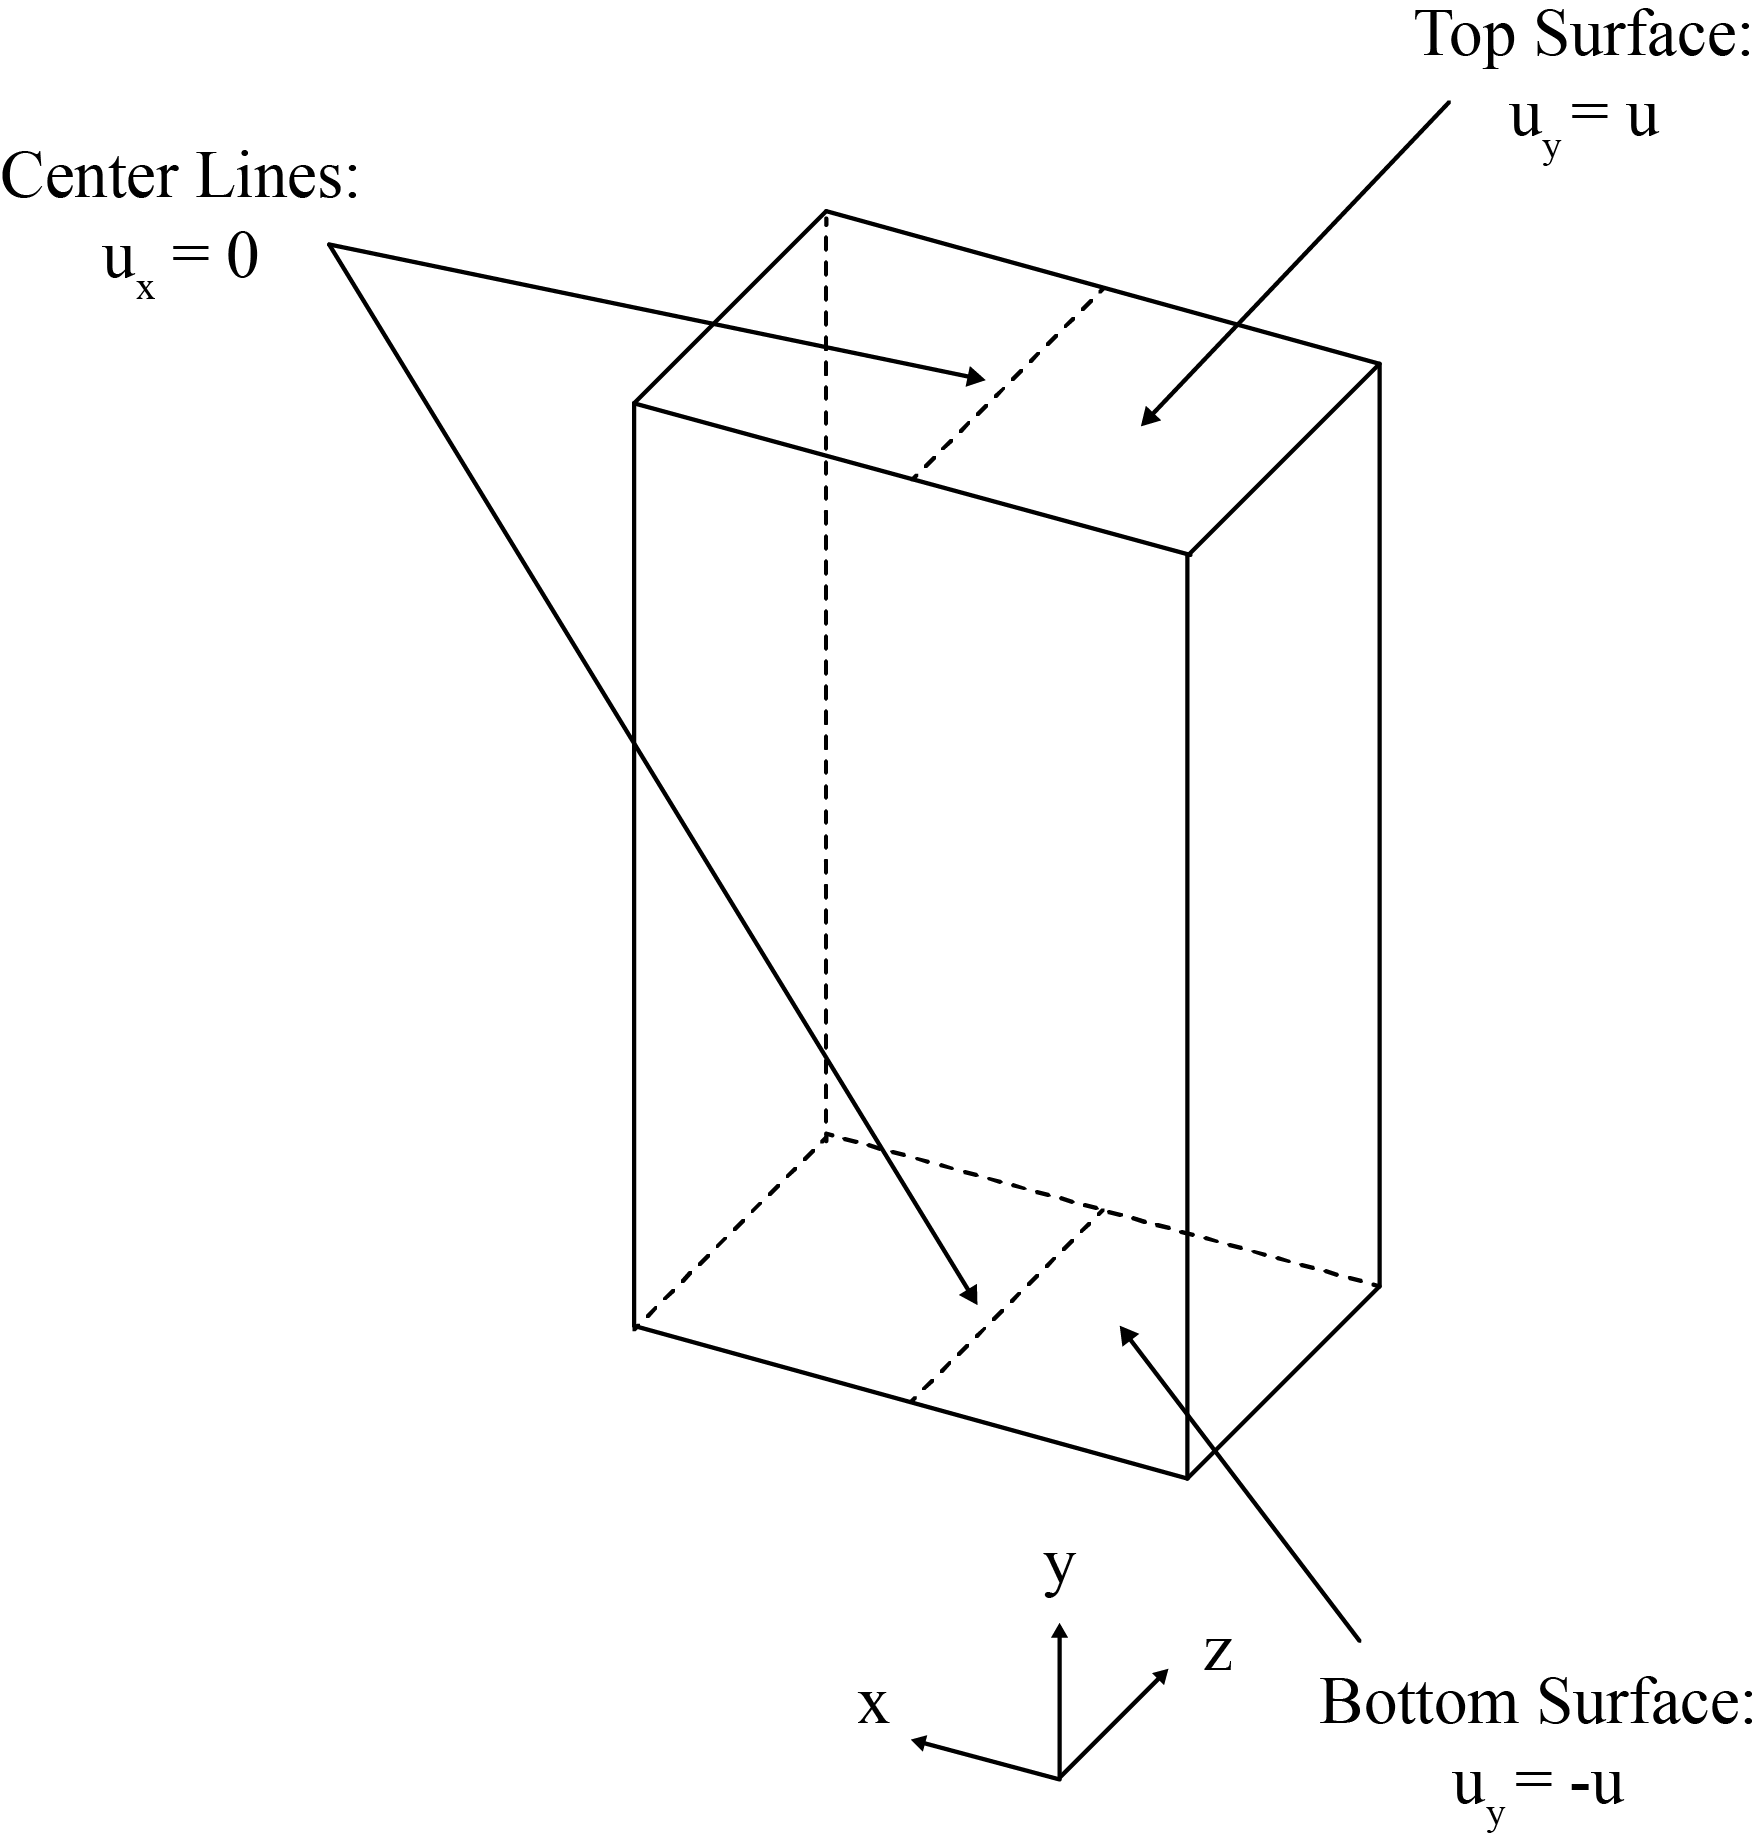
\includegraphics[width=0.6\textwidth]{geometry_figures/BCs.png} }}%
    \qquad
    \subfloat[\centering Model geometry]{{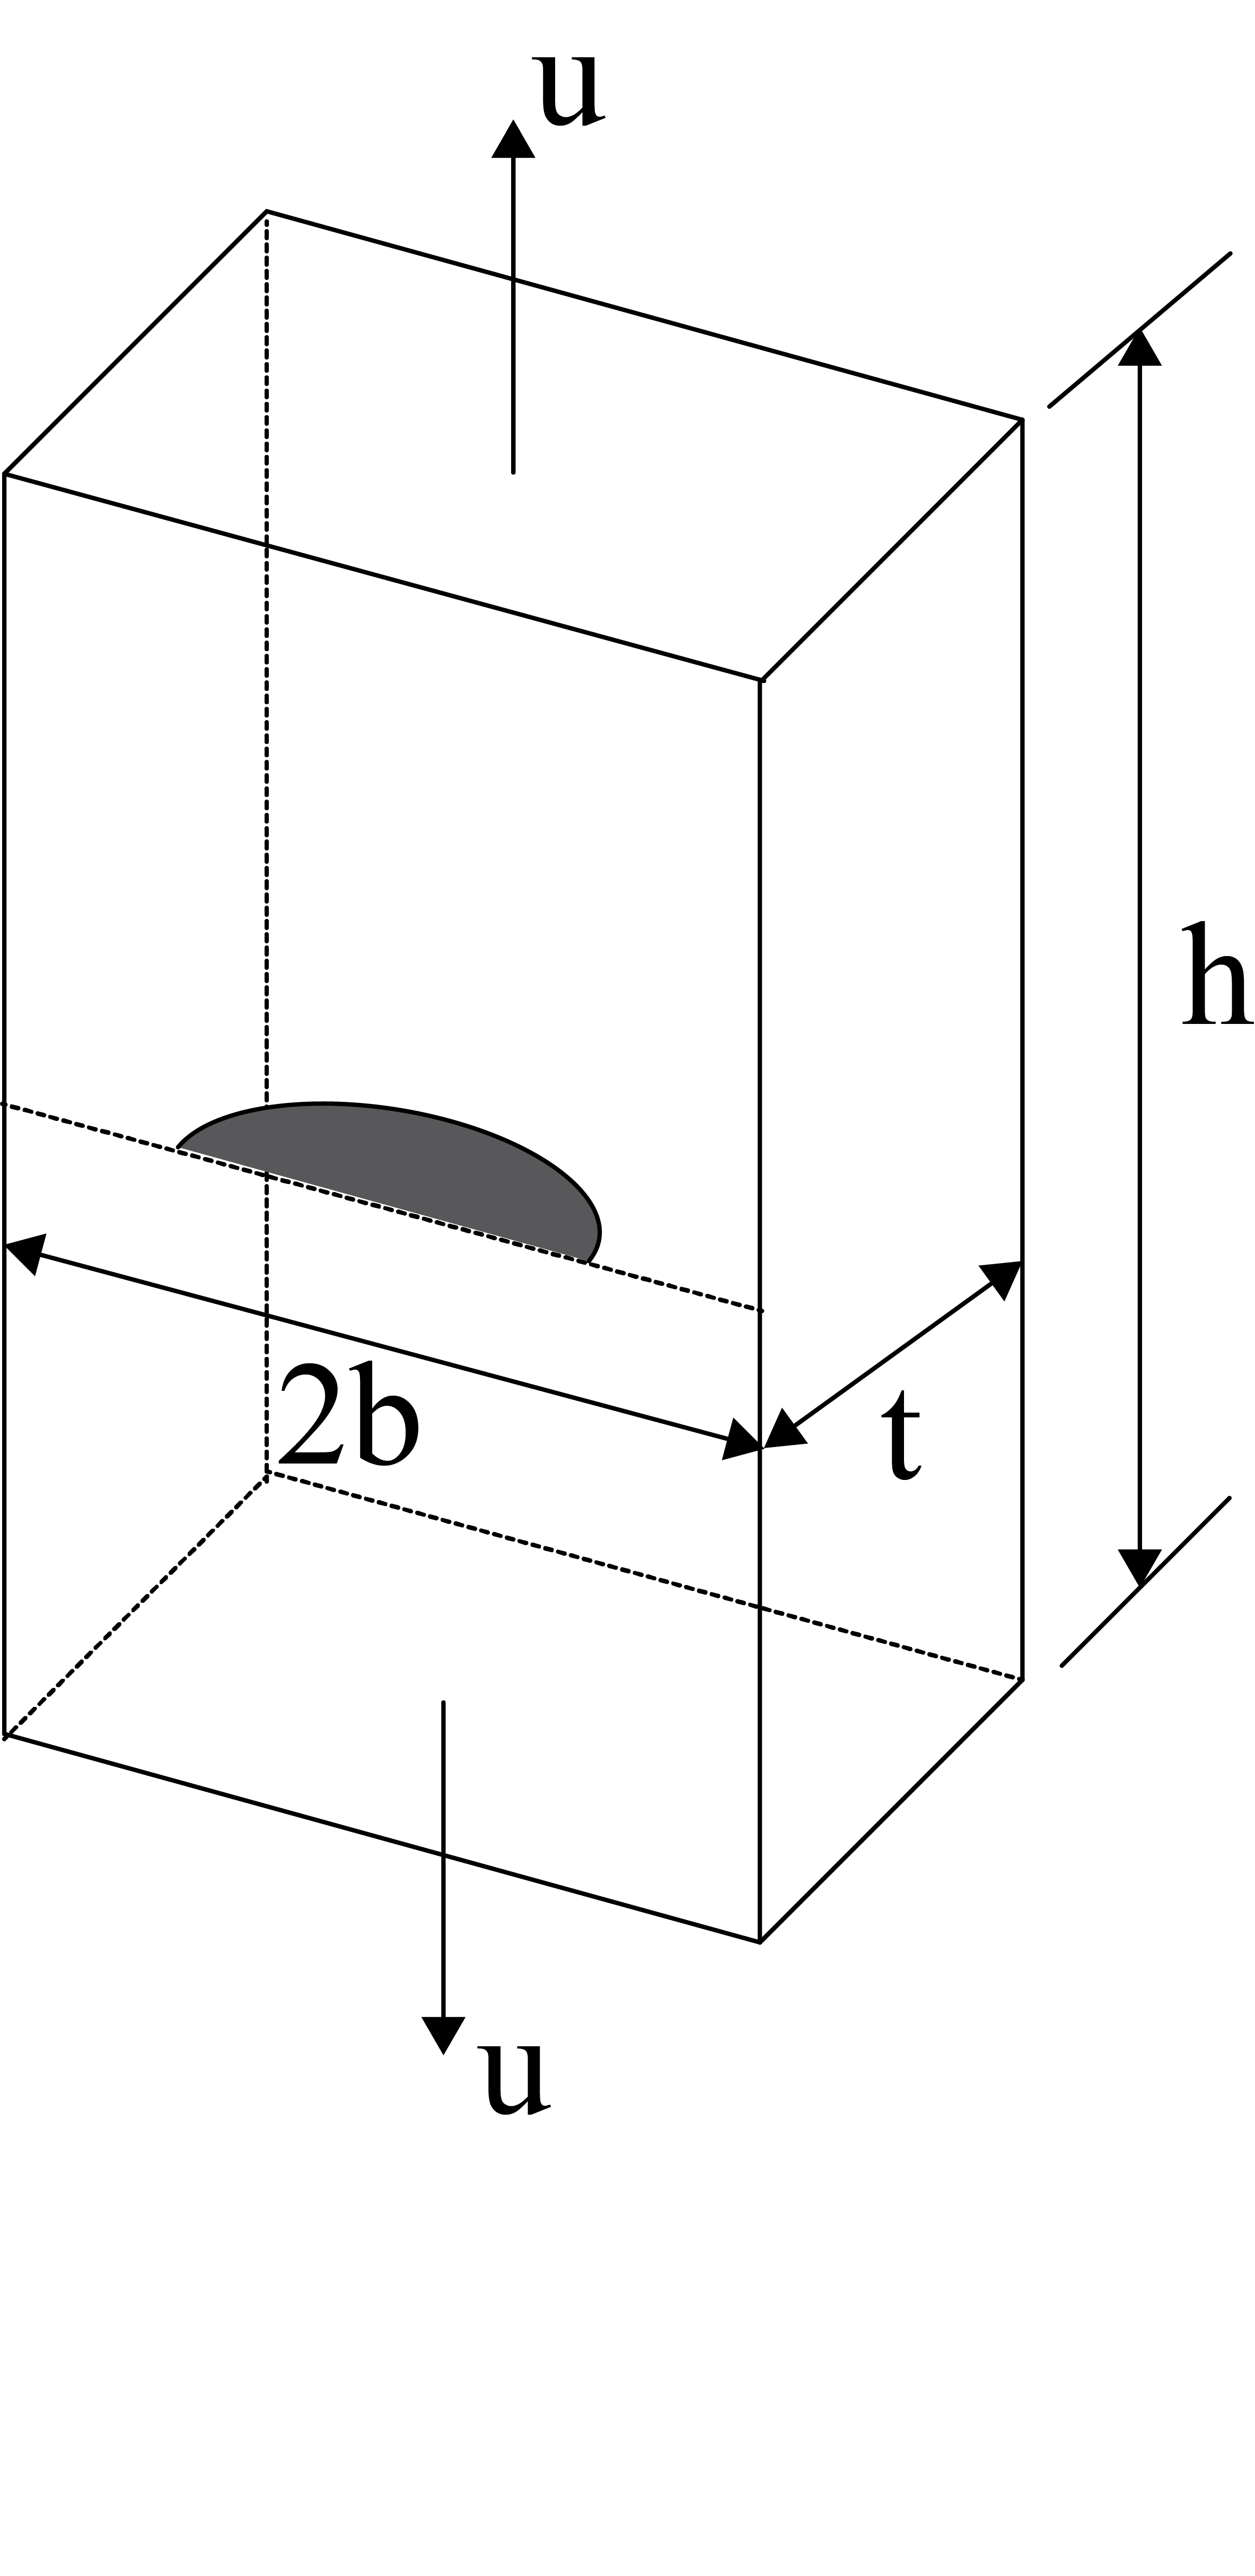
\includegraphics[width=0.3\textwidth]{geometry_figures/Geom.png} }}%
    \caption{(a) Top and bottom surfaces with displacement in $+y$ and $-y$ respectively. The center lines of the top and bottom faces are held at zero displacement in $x$. (b) Model geometry plate height, $h$, plate width, $2b$, and plate thickness, $t$.}%
    \label{fig:model_params}%
\end{figure}
	
%uncracked model
 
\begin{figure}
    \centering
    \subfloat[\centering Convergence of $h/t$]{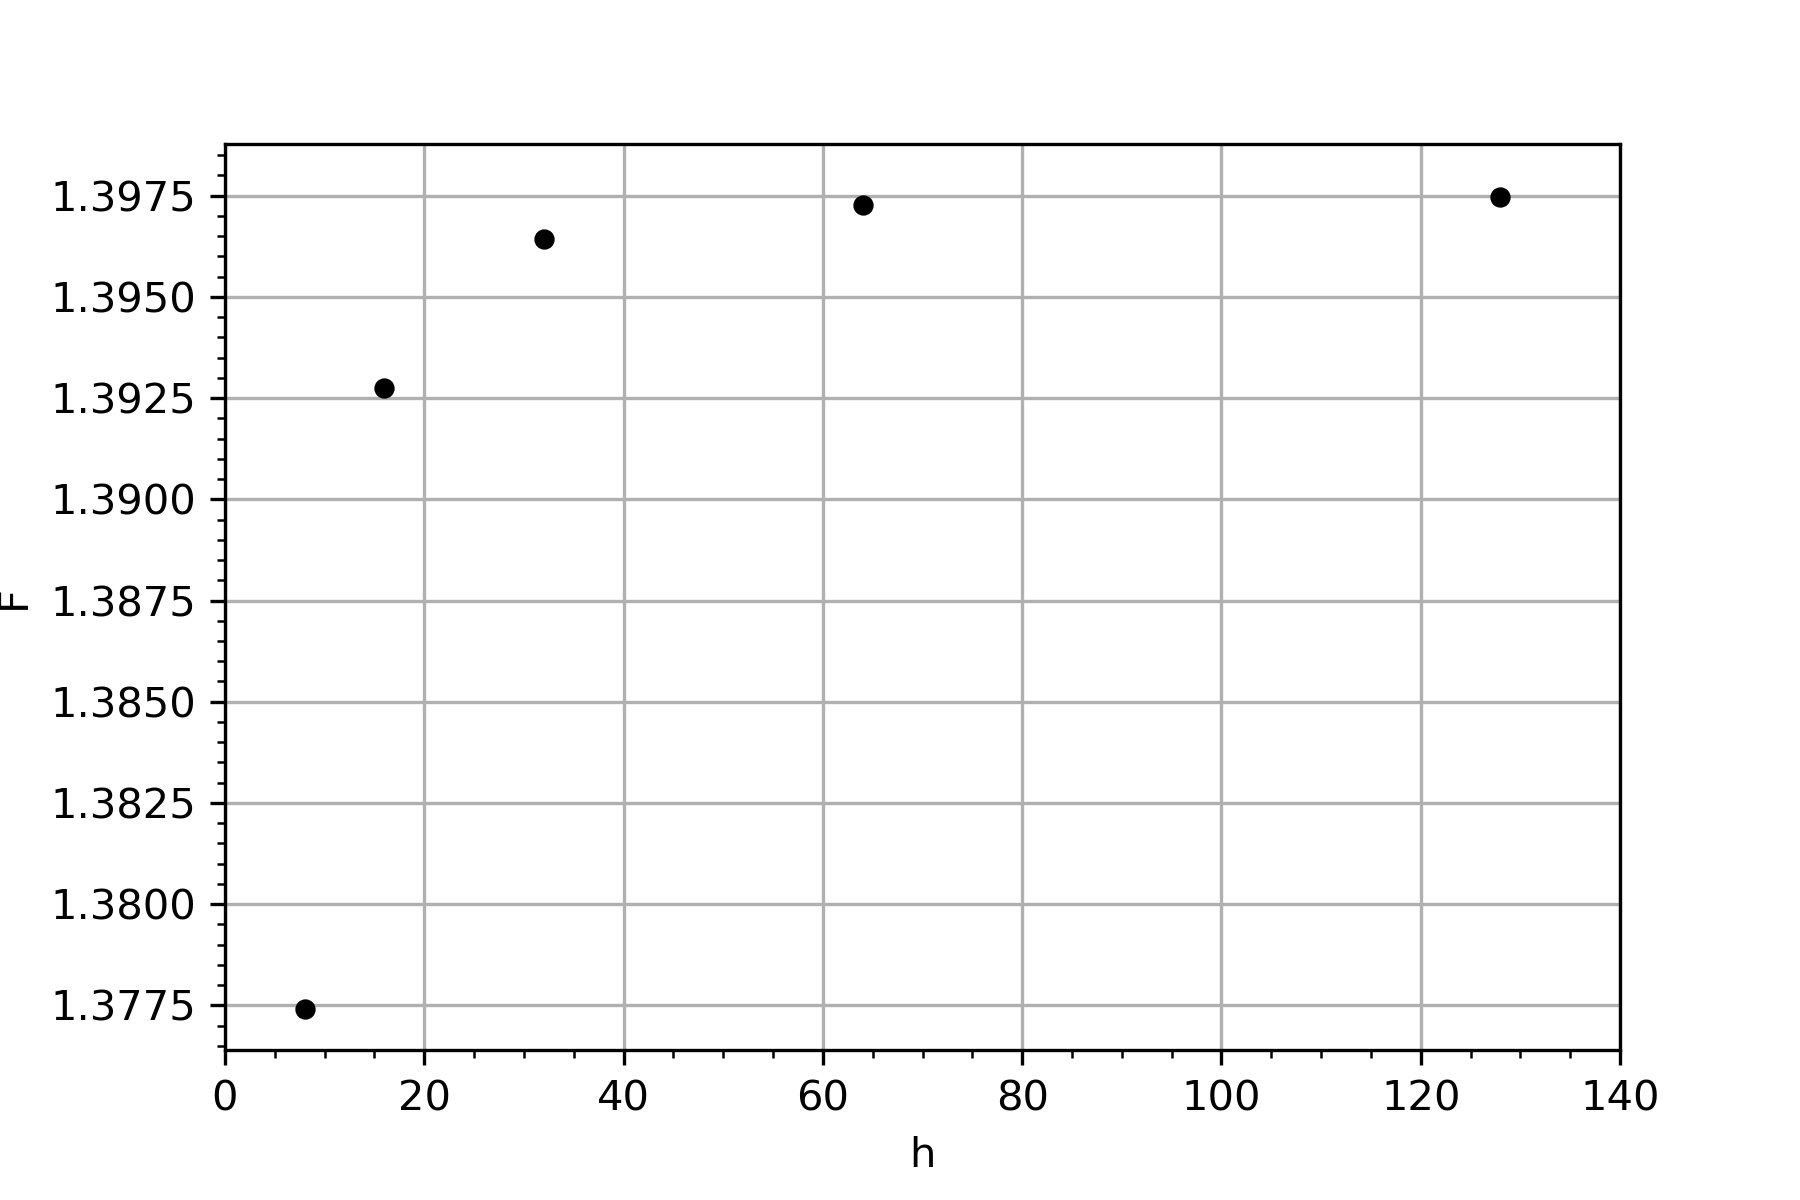
\includegraphics[width=0.45\textwidth]{Figures/h_convergence.png}\label{fig:h_convergence}}%
    \qquad
    \subfloat[\centering Convergence of $c/b$]{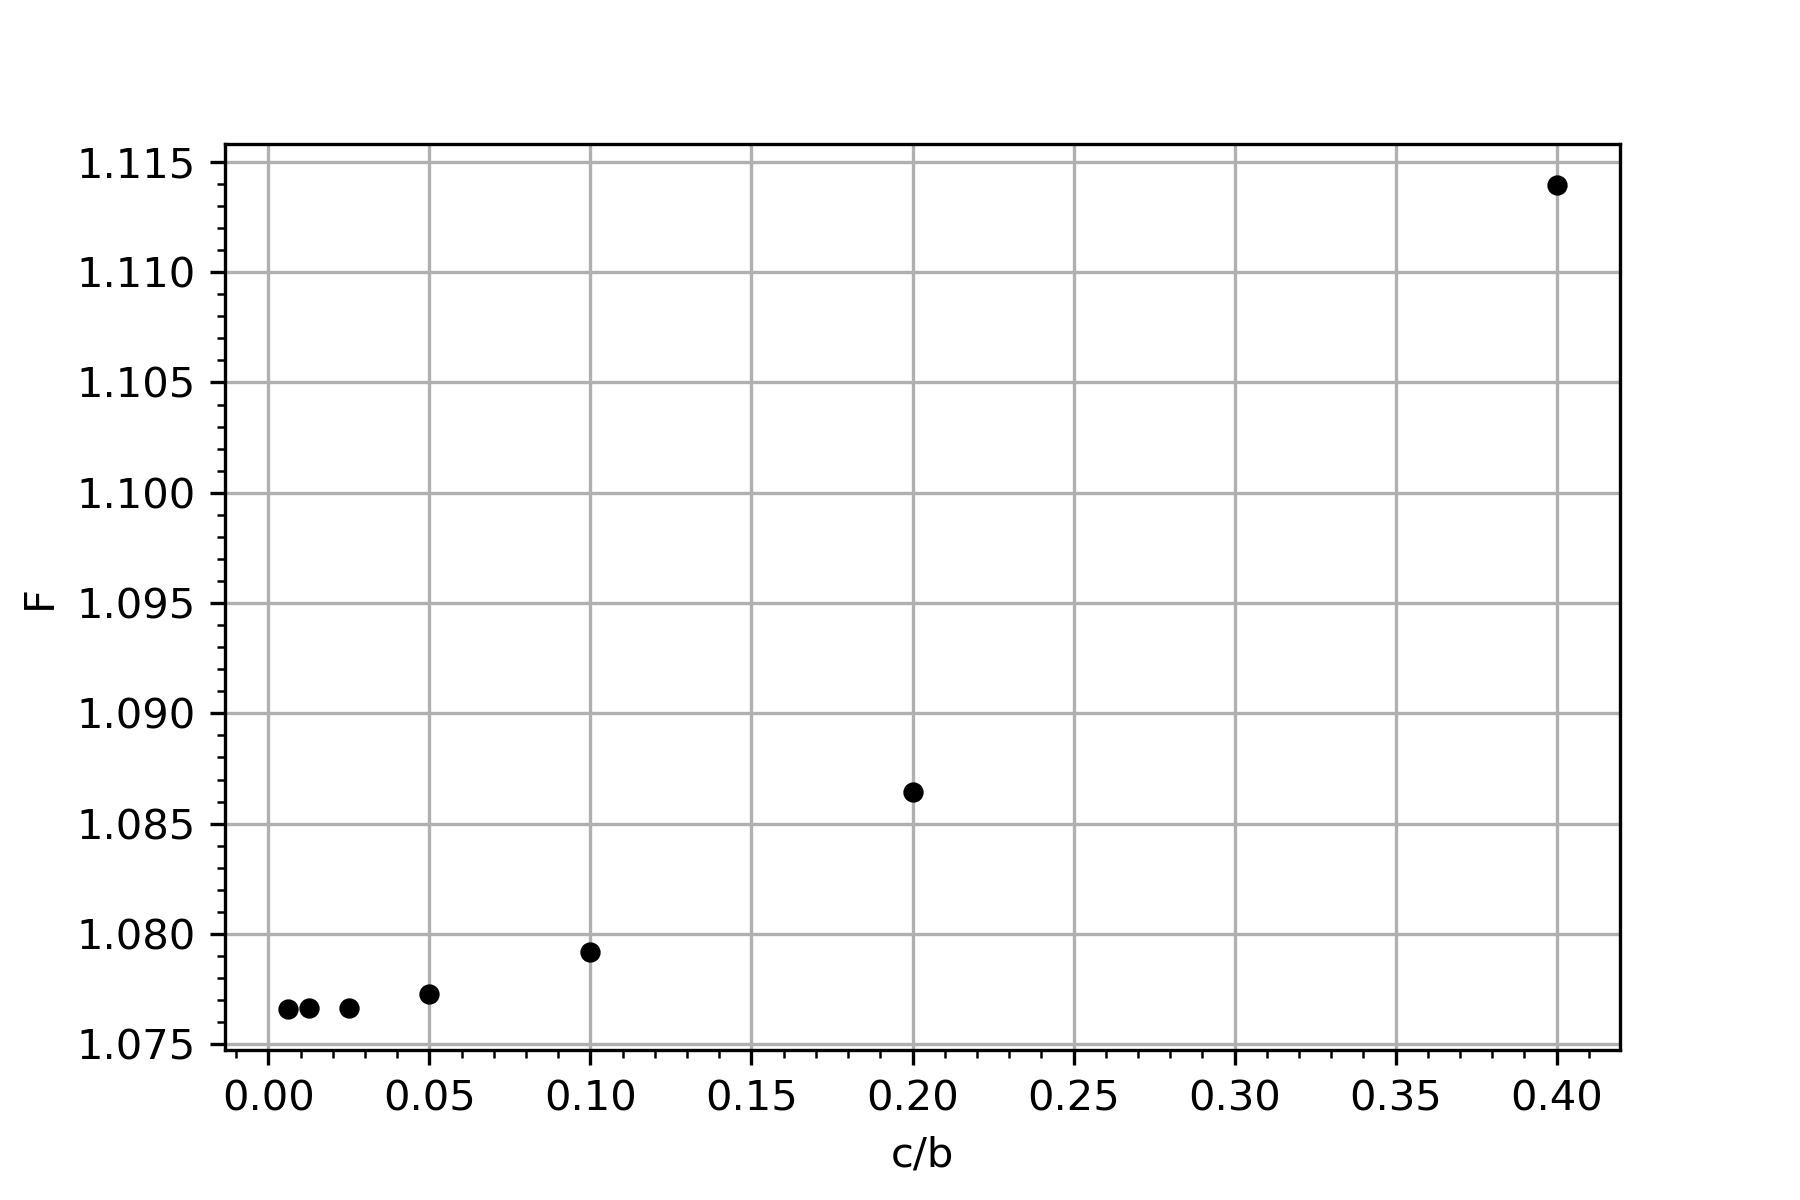
\includegraphics[width=0.45\textwidth]{Figures/cb_convergence.png}\label{fig:cb_convergence}}
    \caption{(a) The convergence of $h/t$ is plotted using the mean *******boundary correction factor. (b) The convergence of $c/b$ is plotted using the mean boundary correction factor.}
    \label{fig:convergence_plots}
\end{figure}

\begin{table}[]
\centering
\begin{tabular}{|l|l|l|l|}
\hline
\textbf{Feature} & \textbf{min} & \textbf{step} & \textbf{max} \\ \hline
a/c              & 0.2          & 0.05          & 2            \\ \hline
a/t              & 0.2          & 0.05          & 0.8          \\ \hline
c/b              & 0.01         & 0.05          & 0.4          \\ \hline
$\phi$           & 0            & $\pi / 150$  & $\pi$        \\ \hline
\end{tabular}
\caption{Max and min values for each of the features used when creating the cracked FE models}
\label{table:feat_range}
\end{table}


The crack mesh template created by FRANC3D is shown in \ref{fig:f3d_crack}. The mesh contains a ring of quarter points elements around the crack front followed by rings of brick elements. The parameters for the crack mesh are the template radius which specifies the size of each element; the number of rings of elements around the crack; and the number of circumferential elements in each ring. Instead of using a fixed template radius a number of elements along the entire crack was specified. This produced better results with varying crack aspect ratios. The best SIF values were computed with 300-600 elements along the crack, 8 rings of elements, and 14 circumferential elements per ring as shown in table \ref{table:optimized_vals}. The average SIF value for each model is relatively insensitive to the crack mesh, however certain crack geometries display numerical noise for certain crack mesh sizes as shown in figure \ref{fig:crack_mesh_convergence}. The models that displayed the most numerical noise for the most crack sizes were the models with values close to the following: $a/c = 0.5$, $a/t = 0.6$, and $c/b = 0.2$. The crack mesh parameters were chosen based off of these models and then applied to the rest of the models. Before running the entire set of training simulations, a random sample of 10\% of the total models was computed to check for convergence. After convergence was confirmed on those models the entire training set was computed. 

\begin{figure}
    \centering
    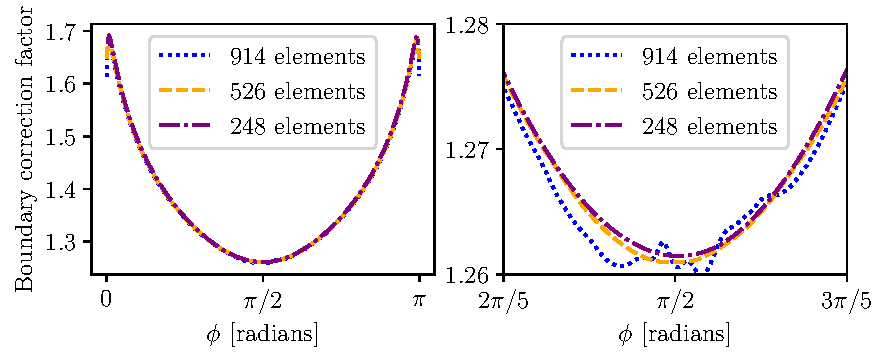
\includegraphics[width=\textwidth]{Figures_pdf/numerical_noise.pdf}
    \label{fig:crack_mesh_convergence}
    \caption{(left) entire SIF plot for differing number of elements along the crack front. (right) plot zoomed in at $\pi/2$ to highlight numerical noise with high element count.}
\end{figure}



The converged values are tabulated in table \ref{table:optimized_vals}
\begin{table}[]
\centering
\begin{tabular}{|l|l|}
\hline
Thickness                   & 1         \\ \hline
h/t                         & 64        \\ \hline
Global seed                 & max(0.25, min(b/50, 0.5))      \\ \hline
Local seed                  & 0.25      \\ \hline
Number of rings             & 8         \\ \hline
Number of circumferential elements             & 14        \\ \hline
Number crack front elements & $\sim$300 \\ \hline
\end{tabular}
\caption{Optimized model and mesh values}
\label{table:optimized_vals}
\end{table}




After the converged model parameters were found all 2500 of the models were run to calculate 300-450 SIFs per model. Figure \ref{fig:selected_sifs} shows the calculated SIF values from a few of the models compared to the SIFs calculated from \cite{RNFEM}.  

\begin{figure}
    \centering
    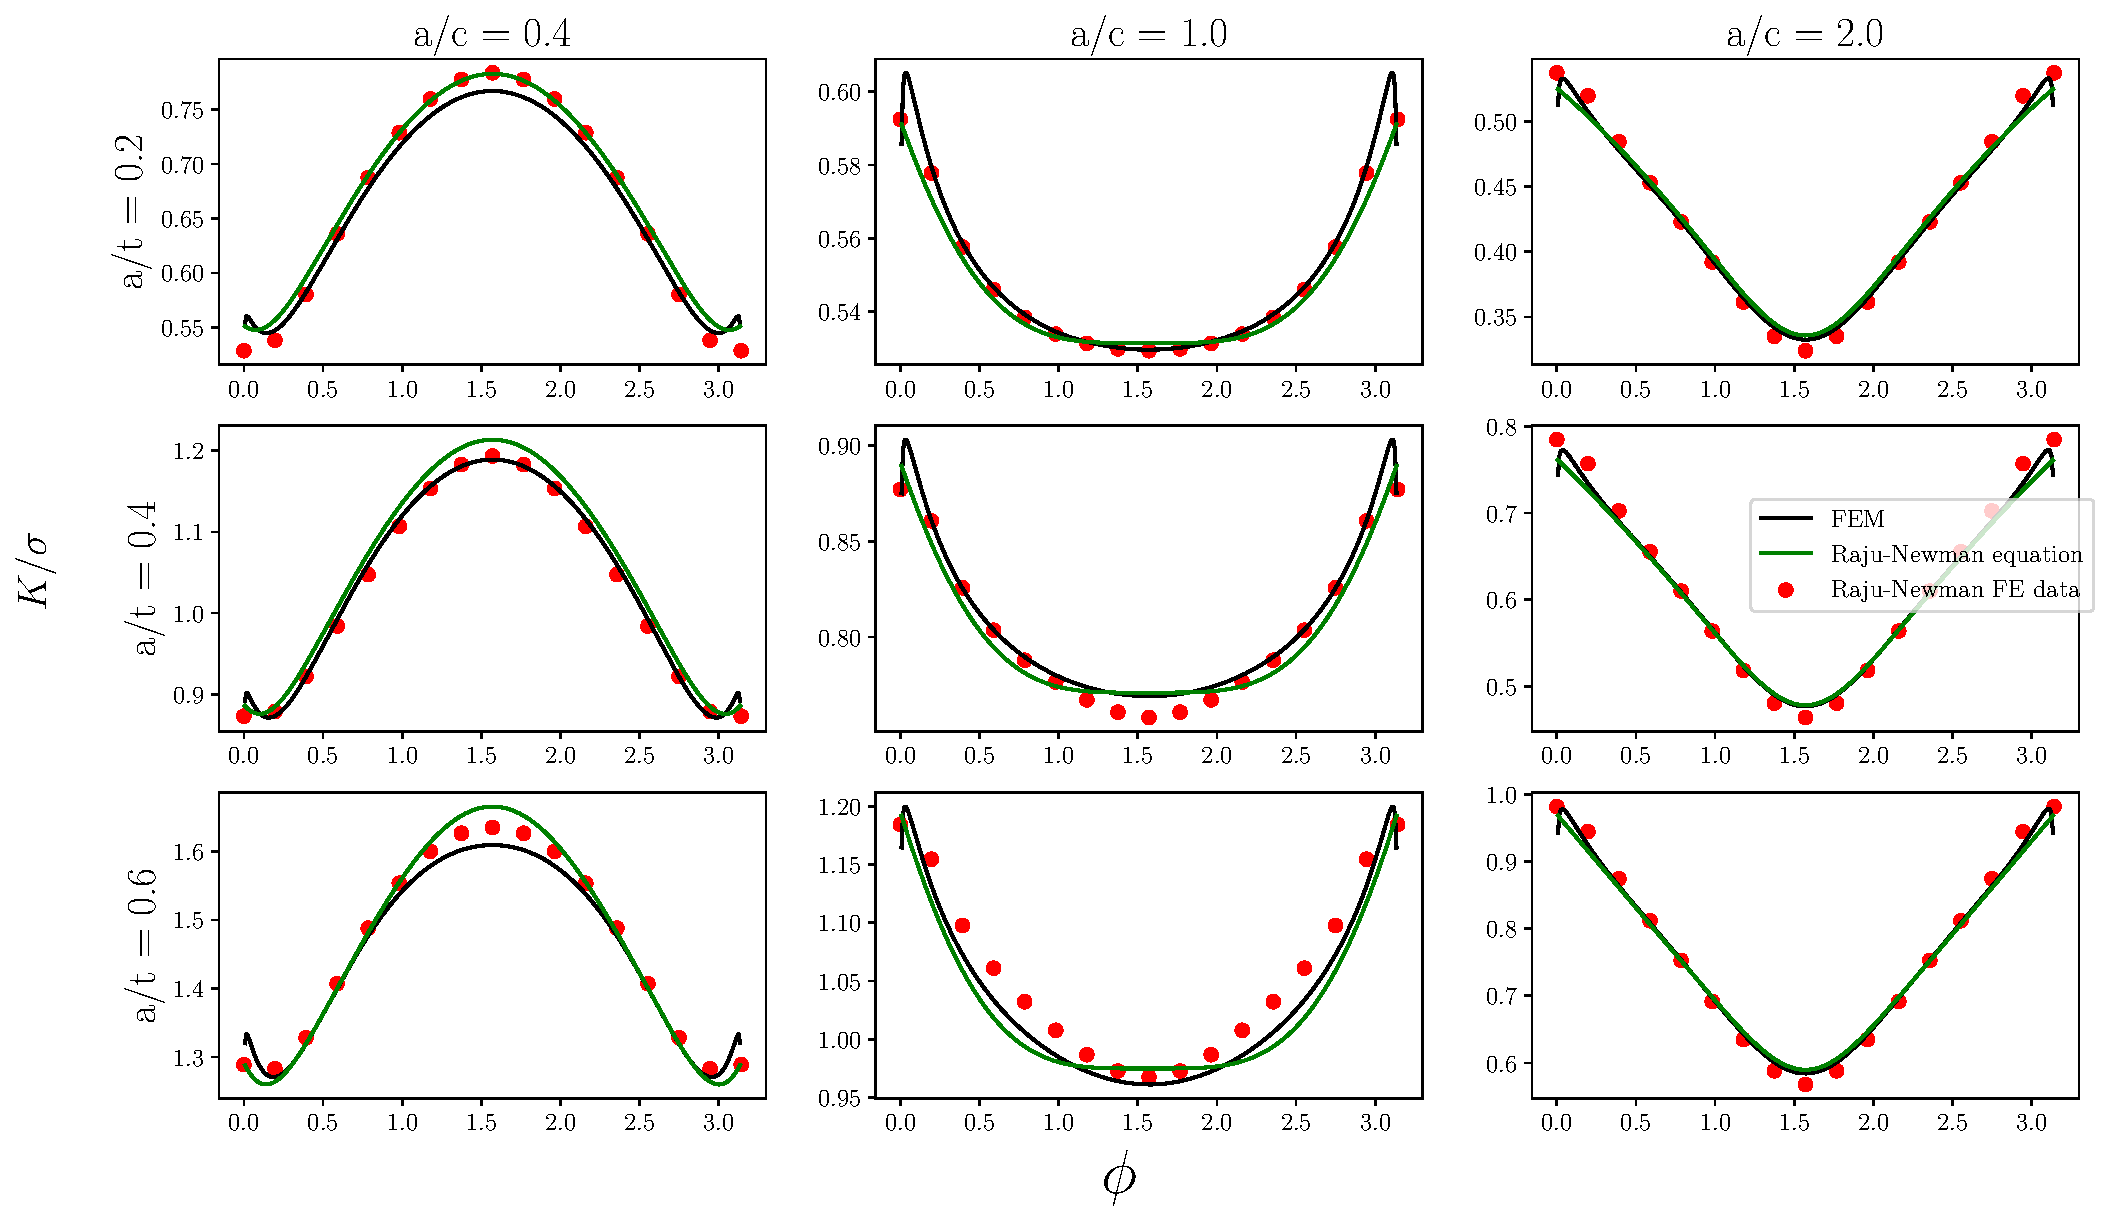
\includegraphics[width=\textwidth]{Figures_pdf/K_data.pdf}
    \label{fig:selected_sifs}
    \caption{SIF values from a selection of models plotted with the Raju-Newman equation.}
\end{figure}

%%%%%%%%%%%%%%%%%%%

\subsection{Training Data Subdivision}

The 2500 training simulations were used for training and model selection, while a additional isolated set of 400 models were generated for testing to allow for better generalization error assessment. Instead of simply training on all of the SIF data at once we use a mechanics based approach to improve the training process and the explainablity of the final produced GPSR SIF model. The general approach used by Raju and Newman \cite{RNeqnsbook} was used to decompose the model for $K$ into two parts: an a priori known part and a learned part. The known part includes Eq. \ref{eqn:K_embedded_ellipse}, which is the solution to the embedded ellipse in an infinite volume. The learned part of the model are the boundary correction factors which are $f_w$, $M$, and $g$ each accounting for a specific correction to the known part. The finite width correction factor, $f_w$, accounts for the effect of finite width and thickness at $\phi = \pi/2$ in a semi-circular crack. $M$ accounts for the aspect ratio of the crack. The two functions $f_w$ and $M$ together comprise the boundary correction factor at $\phi = \pi/2$ along a semi-elliptical crack in a finite plate. Finally $g$ applies this correction at $\phi = \pi/2$ along the crack front allowing for SIFs to be modeled along the entire crack front.
\begin{comment}
	GPSR is especially suited for this process as it finds closed form equations which can conform exactly to the known limits of each of the boundary correction terms significantly increasing interpretability.
\end{comment}
 

Two modifications were made to the approach used in \cite{RNeqnsbook} to both simplify and generalize the training process. First, we extend the definition of the major and minor axes of an ellipse by using the function $l$ from \cite{tada1985} and modifying it to allow for values of $a/c > 1$ Eq. \ref{eqn:l}.


\begin{equation} \label{eqn:l}
l = a \left( \frac{c}{\alpha} \right)^2 \sqrt{\left( \frac{a}{c} \right)^2 \cos^2 \phi + \sin^2 \phi},
\end{equation}

where $a$ is the crack depth, $c$ is half-crack surface length, and $\alpha$ is the length of the major axis of the ellipse. The function $l$ is a measure of the perpendicular distance from the tangent line at the point of interest to the nearest axis seen in figure \ref{fig:crack_params}. The benefit of modifying the embedded ellipse equation by using equation \ref{eqn:l} is that it removes the need for piece-wise functions, Eqns. \ref{eqn:fphi} and \ref{eqn:RN_M1 - eqn:RN_g}. This approach reduces the number of models that have to be trained and lowers the complexity of the final $K$ solution resulting in a more interpretable equation. 

The second modification is the formulation of $f_w$. While Raju and Newman \cite{RNeqnsbook} used a finite width correction factor for a 3d through crack from \cite{brown1966}, this work uses a finite width correction factor for the case of a semi-elliptical surface crack. $f_w$ is still a finite width and thickness correction when $\phi = \pi/2$ and $a/c = 1$. However, unlike Raju and Newman \cite{RNeqnsbook}, by noting that when  $\phi = \pi/2$ and $a/c = 1$ the value of $K$ converges to the embedded ellipse equation as $a/t$ and $c/b$ go to zero, Fig \ref{fig:fw_convergence}.

\begin{figure}
    \centering
    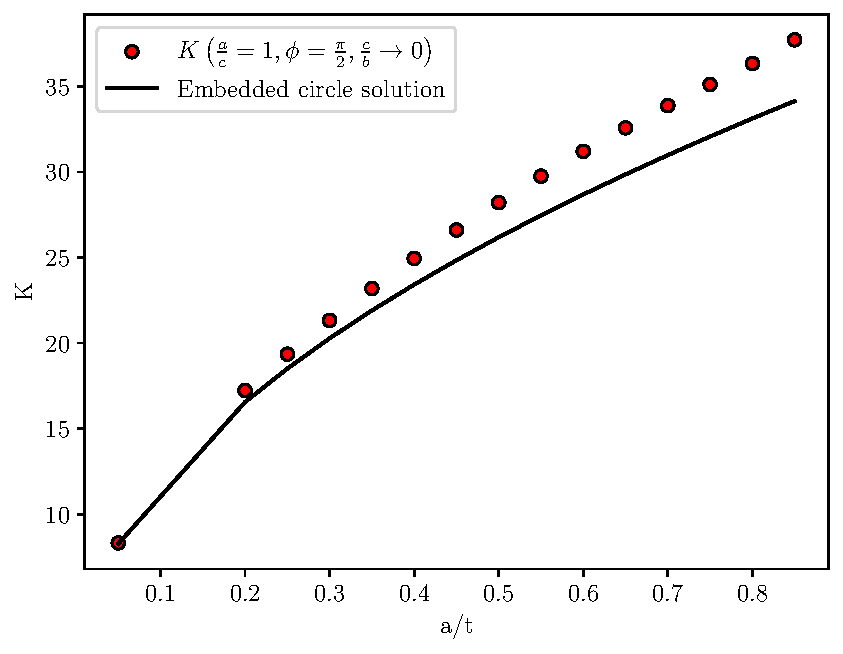
\includegraphics[width=\textwidth]{Figures_pdf/fw_convergence.pdf}
    \label{fig:fw_convergence}
    \caption{Comparison of K from the center of a surface crack and the solution to an embedded circle crack in an infinite volume as a function of a/t where c/b = 0.01. \ref{fig:convergence_plots}}
\end{figure}

The final equation for K is then

\begin{equation} \label{eqn:fw_parameter_def}
    f_w\left(\frac{c}{b}, \frac{a}{t}\right) = \frac{K\left(\frac{a}{c} = 1, \phi = \frac{\pi}{2}\right)}{\sigma \frac{2}{\pi} \sqrt{\pi a}},
\end{equation}



\begin{equation} \label{eqn:K_semi_with_l}
    K = \sigma \frac{\sqrt{\pi l}}{E} f_w M g,
\end{equation}

where $f_w$, $M$, and $g$ are the boundary correction functions learned by using Bingo and $\sigma \sqrt{\pi l}/E$ is the modified embedded ellipse solution. 


A decomposition of training data will now follow the defined correction functions and they dependence on geometric variables as 
\begin{equation} \label{eqn:K_parameter_def}
    K\left(\frac{a}{c}, \frac{a}{t}, \frac{c}{b}, \phi, \sigma \right) = K_{ee} \left(
\frac{a}{c}, \sigma, \phi \right) f_w \left(\frac{a}{t}, \frac{c}{b} \right) M \left(\frac{a}{t}, \frac{a}{c} \right) g \left(\frac{a}{t}, \frac{a}{c}, \phi \right)
\end{equation}

 The next step is to extract the training data for $M$, which is computed similar to $f_w$. Specifically, The SIF training data from FEA simulations are taken at $c/b = 0$ and $\phi = \pi/2$ then normalized by Eqns \ref{eqn:K_embedded_ellipse} and \ref{eqn:fw_parameter_def} as

\begin{equation} \label{eqn:M_parameter_def}
    M \left(\frac{a}{t}, \frac{a}{c} \right) = \frac{K_{FE}\left(\frac{c}{b} \rightarrow 0, \phi=\frac{\pi}{2}\right)}{f_w\left(\frac{c}{b} \rightarrow 0\right) K_{ee}\left(\phi = \frac{\pi}{2} \right)}.
\end{equation}

The final step is to extract the training data for $g$. This is done by normalizing by Eqns\ref{eqn:K_embedded_ellipse, eqn:fw_parameter_def, eqn:M_parameter_def} as

\begin{equation} \label{eqn:g_parameter_def}
    g \left(\frac{a}{t}, \frac{a}{c}, \phi \right) = \frac{K_{FE}\left(\frac{c}{b} \rightarrow 0\right)}{K_{ee} f_w\left(\frac{c}{b} \rightarrow 0\right) M }.
\end{equation}

Forcing $g$ to only be defined at $c/b=0$ matches the Raju-Newman equations. Additional models were trained where $g$ is allowed to be a function of $c/b$ for a more accurate SIF model.



\subsection{Training Bingo Models}

Due to the mechanics based break down of training data in Eqns. \ref{eqn:fw_parameter_def, eqn:M_parameter_def, eqn:g_parameter_def} a reduced subdomain of the feature space is used for training. The function $f_w$ is trained on data where $a/c = 1$ and $\phi = \pi/2$. The function $M$ is trained on data where $c/b = 0$ and $\phi = \pi/2$. The function $g$ is trained on data where $c/b = 0$. Fig. \ref{fig:training_models_3d} shows this training data reduction. In this figure each point represents a FE simulation, each having SIF values along the crack front, $\phi$. One of the simplifications Raju and Newman used when decomposing the SIF into the correction functions was that the effects of $c/b$ could be modeled by the $fw$ equation, neglecting interaction between $c/b$ and $\phi$. To understand the effect of this assumption an  additional set of Bingo models was trained that allowed $c/b$ to be used in $g$ to model $c/b$ interactions with  $\phi$. These additional $g$ models were trained using the entire (not reduced) data set. The data set reduction was only possible with the assumption that $g$ did not include $c/b$

\begin{figure}
    \centering
    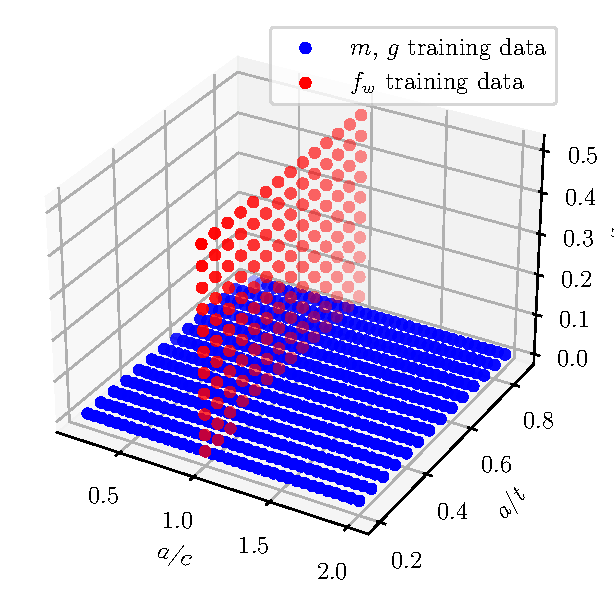
\includegraphics[width=\textwidth]{Figures_pdf/training_slices.pdf}
    \label{fig:training_models_3d}
    \caption{Visualization of the training data reduction allowed by the mechanics based approach. Each point represents a model in the training data-set. $f_w$ was trained when $\phi = \pi/2 \text{ and } a/c = 1$, $M$ was trained when $\phi=\pi/2 \text{ and } c/b = 0$, and $g$ was trained when $c/b = 0$ }
\end{figure}


During the training process, two techniques were employed to improve accuracy and interpretability of the trained $f_w$, $M$, and $g$ models. The first of these techniques involved the use of custom fitness functions to enforce the known constraints  for each model \cite{Hongsup, Karl, Randall2022}. For instance, as the values of $a/t$ and $c/b$ approach zero, the value of $f_w$ converges to 1. A fitness function that calculates the loss when this condition is met and assigns an infinite loss when it is not met enforces the equation's limits. Similar limit constraints apply to $M$ and $g$, such as $M(a/c = 1) = 1$ and $g(\phi = \pi/2) = 1$. The other method used to modify the training process was the addition of seed functions in the initial population. In the initial generation of the Bingo algorithm, a population of randomly generated equations is created. Using seeded equations allows the user to designate a fraction of these randomly generated equations as pre-set equations. This enables users to provide guidance to the algorithm. For example, upon visual examination of the training data for $g$, it was observed that $\left(1 - \sin\phi\right)^{a/t}$ appeared to fit the data well. Additional Bingo models were trained with this function seeded into the initial population. Other Bingo models were trained with only $1 - \sin\phi$ while other had no seeding at all. 

The base fitness function used was mean absolute error. Custom fitness functions were then applied for specific values of $a/c$, $a/t$, $c/b$, and $phi$. For instance as $a/t$ and $c/b$ approach $0$ the values of $f_w$ must approach $1$. This is enforced by checking if the equation inforces the condition and if so it returns the MAE otherwise it returns an infinite loss. The same approach is used for the $M$ and $g$ equations to enforce the known constraints of each model.

The other method of modifying the training process was by the introduction of seed functions \cite{donovan} in the initial population, a population entirely of randomly generated models. For example from the model created by Raju and Newman for $g$ the function  $1-sin\phi$ modeled the bounding conditions on $g$, and we found that $\left(1 - \sin\phi\right)^{a/t}$ modeled the data across its domain. While these seed functions are not required, their definition when known can improve performance. To assess this, we train bingo models with and without these seed functions.

Once the training data has been generated with the described splits and reductions for, $f_w$, $M$, and $g$, can be trained simultaneously. Multiple models were trained for each of the functions, due to the randomness of genetic programming this gave new equations that could be compared to one another to find the best combinations of $f_w$, $M$, and $g$ that predict SIF. The training process is done by first taking the SIF data computed from the FE model and then extracting the $f_w$, $M$, and $g$ training data-sets. Then bingo equations can be found for all three equations, these equation are then combined with the embedded ellipse solution from equation \ref{eqn:K_semi_with_l} to create a prediction for SIFS, this process is visualized in figure \ref{fig:training_flow}.

\begin{figure}
    \centering
    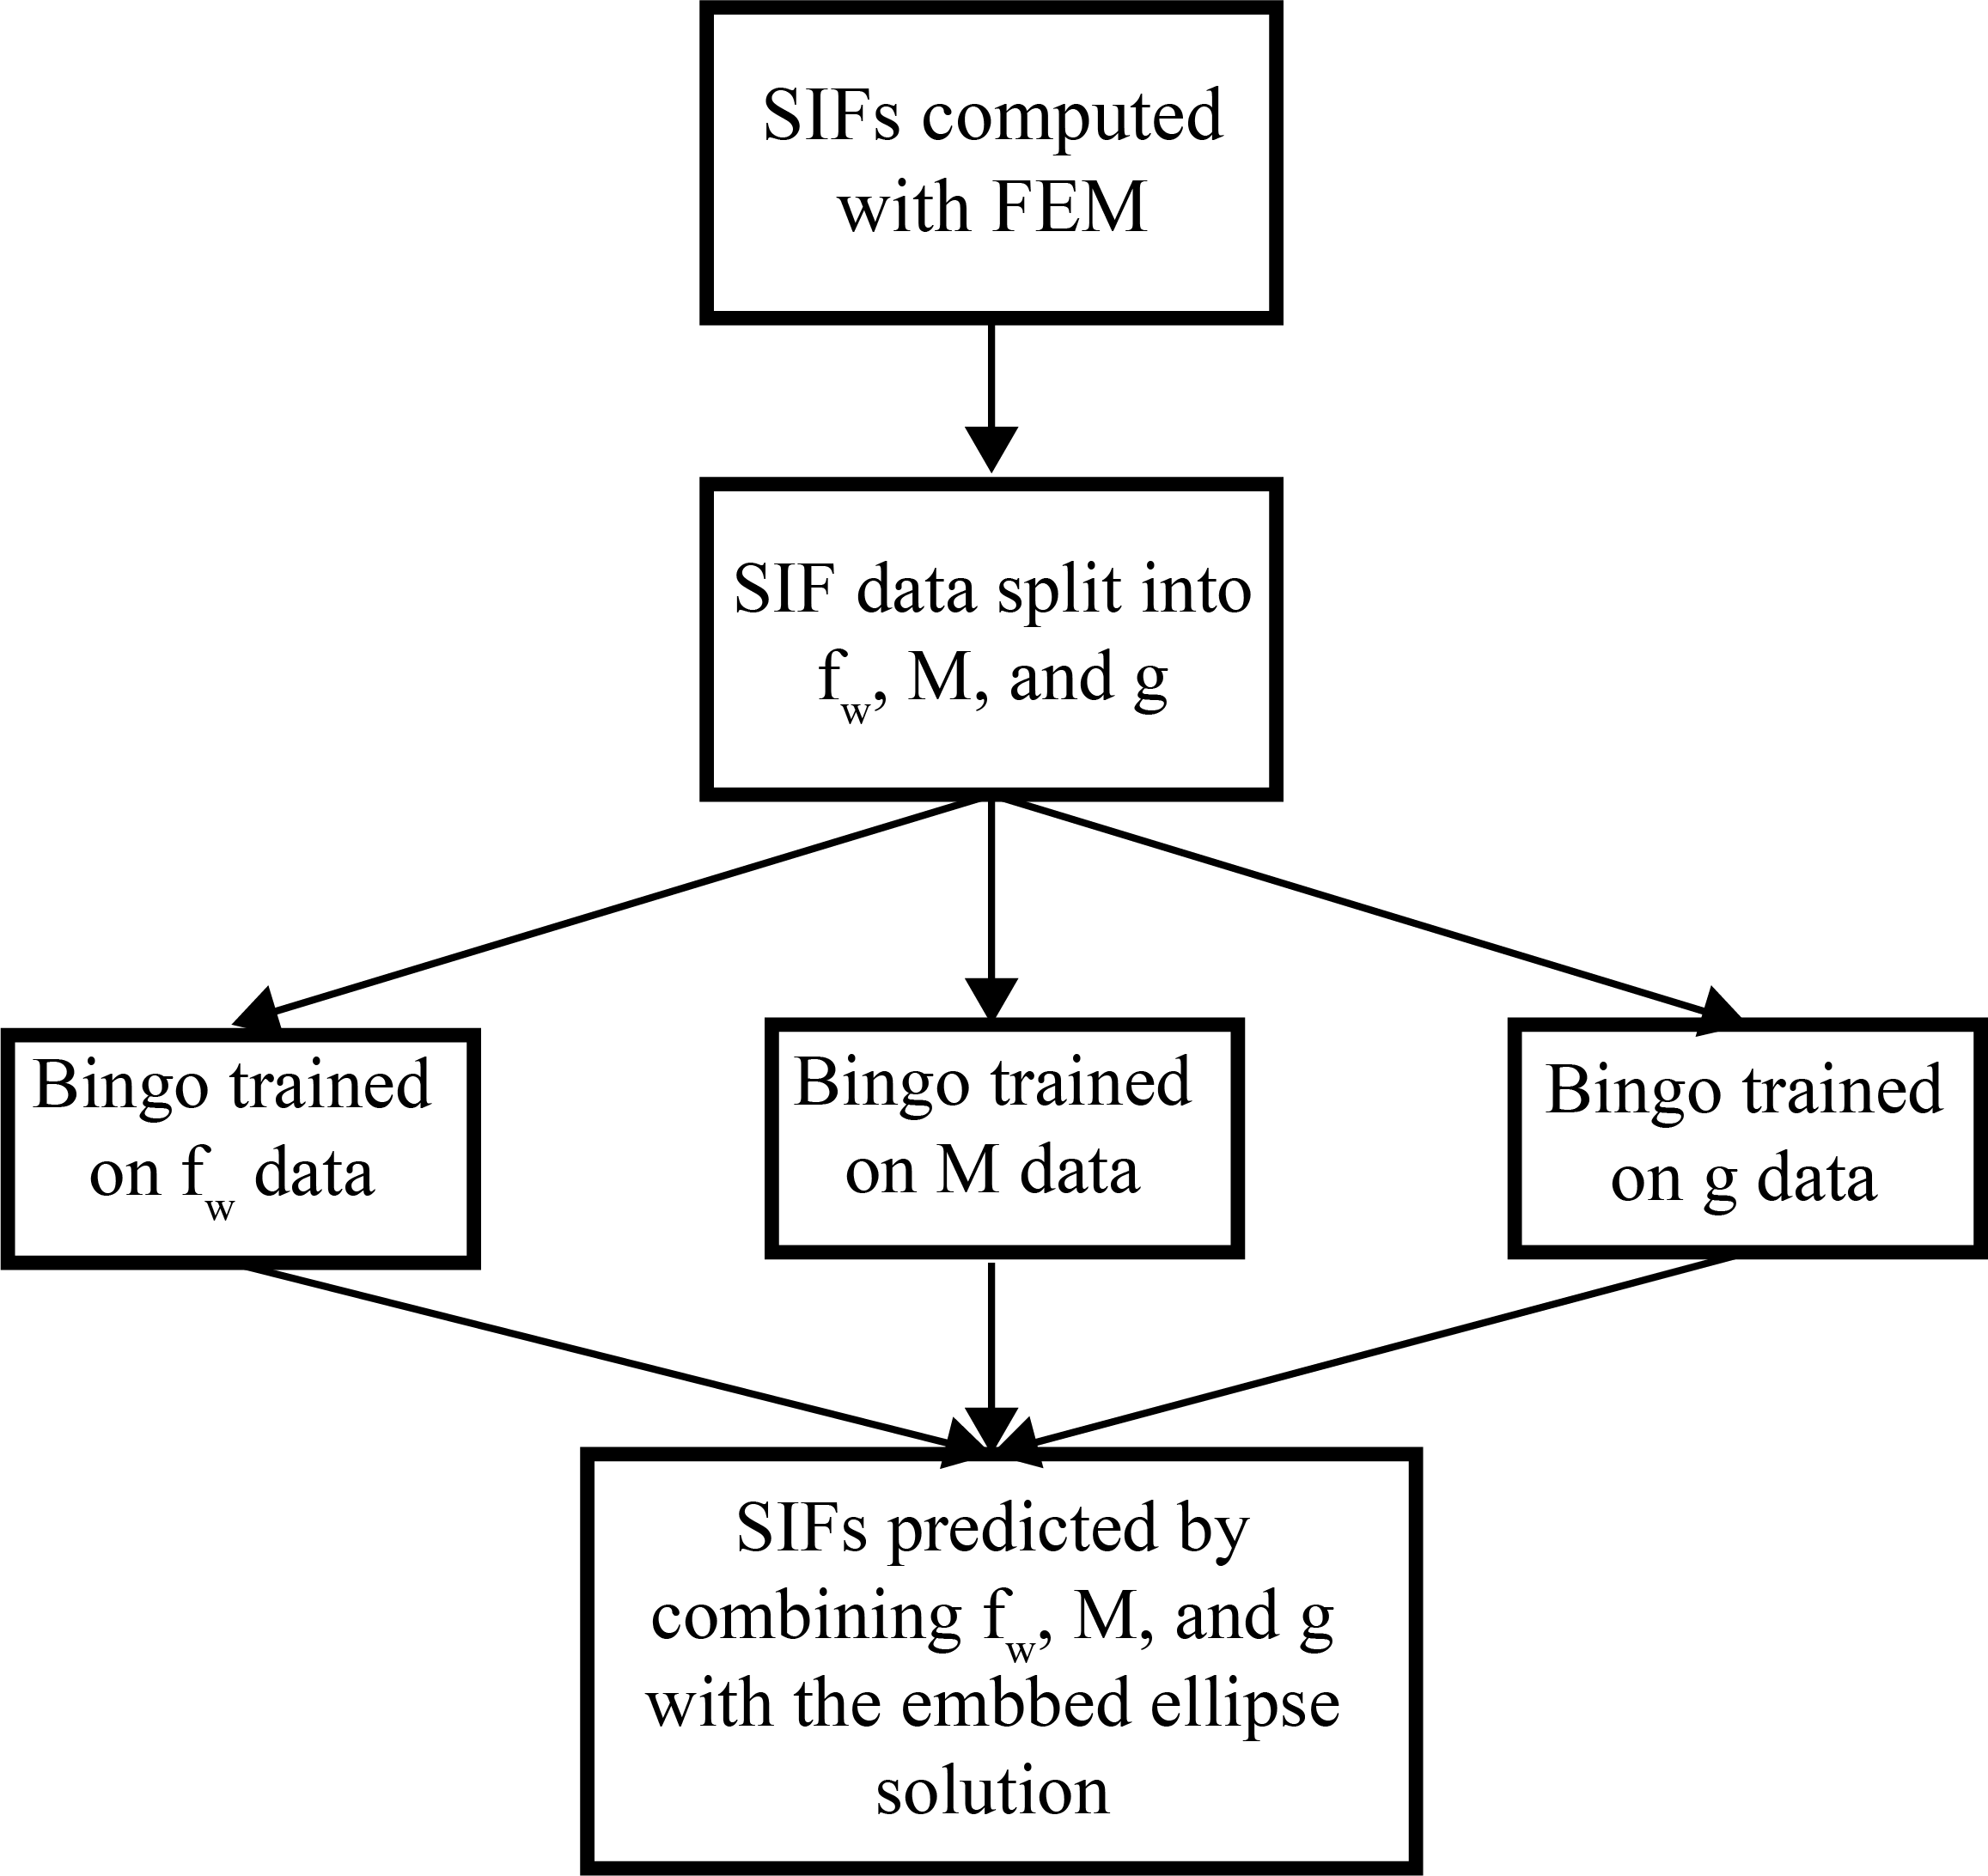
\includegraphics[width=\textwidth]{geometry_figures/training_flow.png}
    \label{fig:training_flow}
    \caption{Flow chart illustrating the training process of the three sub-functions $f_w$, $M$, and $g$}
\end{figure}




